\chapter{Differential Equations}

%%
%% NOTE: This should be an appendix in the future
%%

Differential equations are the fundamental language of dynamical
systems, where they describe how quantities change with time. In
synthetic biology, the quantities of interest might be the
concentration of a particular set of proteins or metabolites or the
concentration of cells and nutrients in a solution of bacteria. When
dealing with a large number of cells, concentrations make sense and we
think of them as continuous. When dealing with single cells where
there may be only 20 of a given protein at a given time,
concentrations do not quite make sense. Nevertheless, many researchers
assume that concentrations are continuous anyway and often arrive at
useful mathematical models. 

In this chapter we look at the basic definitions, examples and
properties of ordinary differential equations. In
Chapters~\ref{ch:mak} (Mass action Kinetics) and ~\ref{ch:enzyme}
(Time Scale Separation) we describe how to derive and analyze
differential equations using modeling assumptions common in synthetic
biology.

The material given in this chapter is meant as a reminder and means to
fix notation. A much more complete introduction to differential equations
and dynamical systems requires a textbook, such as the one by Hirsch
and Smale \cite{hirsch-smale} or \cite{khalil}.

\section{Definitions and Examples}
% definitions

A system of differential equations has the form
%
\begin{eqnarray*}
\dot x_1 & = & f_1 (x_1, ..., x_n, t ) \\
         & \vdots & \\
\dot x_n & = & f_n ( x_1, ..., x_n, t )
\end{eqnarray*}
%
where $t$ is time, $x_1(t), ..., x_n(t)$ are time-dependent {\em state
  variables}, and $f_1, ..., f_n$ are functions. We usally write $x_i$
instead of $x_i(t)$. The notation $\dot x_i$ means $\frac{d}{dt}x_i$. In
vector notation, the above system is more compactly written
%
\begin{equation} \label{eqn:ode}
\dot x = f( x, t )
\end{equation}
%
where $x(t) \in \reals^n$ and $f : \reals^n \times \reals \rightarrow \reals$. 

% examples
  % bacterial growth
  % gene regulation

\begin{example} \label{ex:gene-exp} Suppose that $v_X(t)$ represents
  the concentration of a constitutively expressed protein $X$. Let the
  rate at which the protein is produced be $k_1 > 0$ and the rate at
  which it is degraded be $k_2 > 0$. Using these two parameters, a
  (very) simple model of protein production is then
%
\begin{equation}\label{eqn:gene-exp}
\dot v_X = k_1 - k_2 v_X .
\end{equation}
%
Note the term $-k_2 v_X$ describes the fact that the higher the
concentration of $X$, the more ``degradation events'' occur per
minute. The production of $X$ described by the $k_1$ term, on the
other hand, is indpendent of how much $X$ there already is in the
system. \enx
\end{example}

\begin{example} \label{ex:growth} Consider a population of of bacteria
  growing in a solution of growth media. The two variables of interest
  are the amount of bacteria $x_1$ (in grams) and the amount of nutrient
  $x_2$ (in grams) in the solution. Monod described the dynamics of this
  situation as follows \cite{monod-growth}.
\begin{eqnarray}
\dot x_1 & = & \frac{v x_1 x_2}{k+x_2} \nonumber  \\
\dot x_2 & = & - \gamma \frac{v x_1 x_2}{k+x_2} \label{eqn:monod}
\end{eqnarray}
where $v$, $k$ an $\gamma$ are parameters. Note that if $x_1=0$ or
$x_2=0$, then there is no growth since there are either no bacteria or
no nutirents. Also notice that as the nutrients $x_2 \rightarrow
\infty$, we get that the growth rate $\dot x_1 \rightarrow v
x_1$. This models the fact that the population cannot grow infinitely
quickly. The parameter $\gamma$ describes the amount of nutrients
needed to make one bacterium. Finally, the parameter $k$ describes the
{\em half-saturation} point, which is the amount of nutrient required
to make $\dot x_1 = v x_1 / 2$. \enx
\end{example}

% solutions
A {\em solution} to the differential equation \eref{eqn:ode} is an explicit
function of time $x(t)$ that satisfies the equation. Explicit
solutions are readily available for some types of differential
equations. For example, equations in which each term appears linearly
are easy to solve. However, for most differential equations, an
explicit solution is difficult or (provably) impossible to find. In
such cases, other analytical techniques must be used. 

\begin{example} \label{ex:gene-exp-sol}
The solution to linear differential equation~\eref{eqn:gene-exp} is 
%
\begin{equation}\label{eqn:gene-exp-sol}
v_X(t) = e^{-k_2 t} \left ( v_X(0) - \frac{k_1}{k_2} \right ) + \frac{k_1}{k_2}
\end{equation}
%
where $v_X(0)$ is the initial concentration of $X$. An explicit
solution such as this tells us almost everything we might want to know
about the behavior of the system. For example, it is easy to see that
as $t \rightarrow \infty$, the concentration $v_X(t) \rightarrow
k_1/k_2$.

In contrast, the differential equation~\ref{eqn:monod} is nonlinear
and has no explicit solution.  \enx
\end{example}

\section{Simulation}

Probably the first thing most analysts do with a new set of
differential equations is simulate them. There are a wide variety of
simulation tools available. For example, one can use the {\tt NDSolve} function
in Mathematica (as described in Appendix~\ref{app:math}) or the {\tt
  ode45} numerical integrator in MATLAB. All of these methods are
based on essentially the same idea. One approximates the state
$x(t+\delta)$ in some way using the state $x(t)$ and the vector field
$f(x,t)$. In this section we breifly describe a simple method of
numerically integrating a set of differential equations, called {\em
  Euler} integration. Once this method is understood, more advanced
methods should make more sense.

In Euler integration, we use the fact that
%
$$
\frac{dx}{dt} = f(x,t) = \lim_{h \rightarrow 0} \frac{x(t+h) - x(t)}{h} \approx  \frac{x(t+\delta) - x(t)}{\delta}
$$
%
when $\delta$ is small. Solving for $x(t+\delta)$ gives
%
\begin{equation}\label{eqn:euler}
x(t+\delta) \approx x(t) + \delta f(x(t),t) .
\end{equation}
%
We then have a simple algorithm.
%
\begin{enumerate}
\item initialize $x_0$, $t_0=0$ and $k=0$
\item while $t_k<t_\mathit{max}$
\item \ \ $x_{k+1} = x_k + \delta f(x_k,t_k)$
\item \ \ $t_{k+1} = t_k + \delta$
\item end while
\end{enumerate}
%
The fidelity of this approximation, and the intensity of the
compuation required, increase as $\delta$ decreases. The next example
illustrates these observations.

\begin{figure}
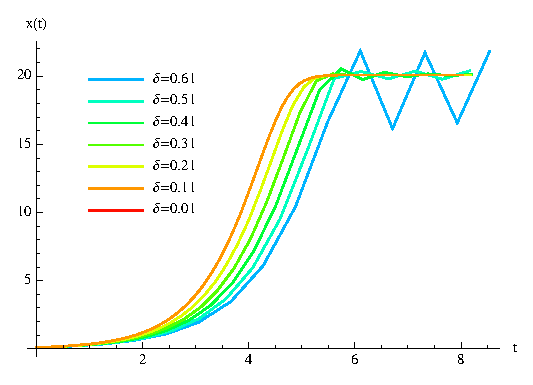
\epsfig{file=figures/euler.eps}
  \caption{\label{fig:euler} Simulations of bacterial growth using Euler integration
    with differing time steps. Large time steps give more results, but
    fewer steps. Smaller time give higher fidelity results.}
\end{figure}

\begin{example}
  Figure~\ref{fig:euler} shows seven simulations of the bacterial
  growth system from Example~\ref{ex:growth} with $v=2$, $k=5$,
  $\gamma=0.5$, $n(0)=10$ and $x(0)=0.1$. Note that the curves for
  $\delta=0.11$ and $\delta=0.01$ are essentially the same. Clearly
  the curves for $\delta \geq 0.21$ are of questionable fidelity. A
  large $\delta$ even introduces oscillations. \enx
\end{example}

\section{Equlibria and Stability}

% equilibria
% local stability
% stability, lyapunov

A state $x^*$ that is a root of $f$, so that $f(x^*,t) = 0$, is
called an {\em equilibrium}. A system may have zero, one or many
equilibria. Solutions to a system may tend toward $x^*$, meaning $x^*$
is stable, or they may veer away from $x^*$, meaning $x^*$ is
unstable. More formally, we are usually concerned with the following
notions of stability. 

\begin{definition} \label{def:stability}
  An equilibrium $x^*$ is {\em locally asymptotically stable} if there
  exists a $\delta>0$ such that 
$$
||x(0)-x^*|| < \delta \; \Rightarrow \; \lim_{t \rightarrow \infty} x(t) = x^* .
$$
If $\delta$ can be anything in the above, then $x^*$ is {\em globally
  asymptotically stable}. 

A system is said to be (locally or globally) {\em exponentially
  stable} if the rate of convergence to $x^*$ is exponential, that is,
if there exist constants $a,b > 0$ such that 
%
$$
||x(t)-x^*|| \leq a ||x(0)-x^*|| e^{-bt}
$$
%
for all $t \geq 0$. 
\end{definition}

\begin{example}
  Suppose that $k_1=1$ and $k_2=1$ in Example~\ref{ex:gene-exp}. The
  dynamics of $X$ are then 
%
$$
\dot v_X = 1 - v_X. 
$$
Setting the derivative equal to zero gives the equilibrium $v_X^* =
1$. As noted in Example~\ref{ex:gene-exp-sol}, the solution is 
%
$$
v_X(t) = ( v_X(0) - 1 ) e^{-t} + 1,
$$
%
which tends toward $1$ exponentially fast as $t \rightarrow
\infty$. Thus, the equilibrium $v_X^* = 1$ is globally exponentially stable. \enx
%
\end{example}

Proving that an equilibrium of a system is stable can be difficult. If
the system is linear, then it is easy. If the system in nonlinear, and
one wants to show local stability, then the system can be linearized
(see below), and the problem becomes easy. Proving that a point is
globally stable is hard, however. Also difficult is characterizing the
region (finding $\delta$ in Def.~\ref{def:stability}) around a locally
stable $x^*$ for which solutions tend toward $x^*$ (i.e. estimating
the {\em region of attraction}). Unfortunately, a point may be locally
stable with a tiny region of attraction.

% lyapunov
The main tool for proving global stability in nonlinear systems is
to use a {\em Lyapunov function}, which is an energy-like function that
decreases on all trajectories of the system as they tend toward the
equilibrium. All stable systems have Lyapunov functions, and if a
Lyapunov function can be found, the system is stable. However, find a
Lyapunov function is difficult, and no efficient method for doing so
can be found. Nevertheless, the method often proves to be useful. 

\begin{theorem} [Lyapunov's Direct Method] \label{thm:lyapunov}
  Consider a system $\dot x = f(x)$ and an equilibrium $x^*$. The
  function $V : \reals^n \rightarrow \reals$ is a {\em Lyapunov Function} if
\begin{enumerate}
\item[i.] $V(x) > 0$ for all $x \neq x^*$;
\item[ii.] $V(x^*) = 0$; and
\item[iii.] $\frac{d}{dt} V ( x ( t ) ) < 0$ for all $x \neq x^*$.
\end{enumerate}
If $V$ is a Lyapunov function, then the point $x^*$ is globally
asymptotically stable.
\end{theorem}

\begin{example} \label{ex:lyapunov}
Consider the system
%
\begin{eqnarray*}
\dot x_1 & = & x_2 \\
\dot x_2 & = & -x_1 - 2 x_2 .
\end{eqnarray*}
%
This system has an equilibrium when $x_1=x_2=0$. Now define
$V(x_1,x_2) = \frac{1}{2} ( x_1^2 + x_2^2 )$ to be a {\em candidate}
Lyapunov Function. Clearly conditions (i) and (ii) in
Theorem.~\ref{thm:lyapunov} hold. For the third condition,
%
\begin{eqnarray*}
\frac{d}{dt} V & = & \frac{d}{dt} ( x_1^2 + x_2^2 ) / 2 \\
               & = & x_1 \dot x_1 + x_2 \dot x_2 \\
               & = & x_1 x_2 + x_2 ( -x_1 - 2 x_2 ) \\
               & = & - x_2^2 < 0 
\end{eqnarray*}
%
when $x \neq 0$. We can therefore safely assume that no matter what
the initial condition, this system always converges to $0$. \enx
\end{example}

One way to visualize what at least a two-dimensional system behaves
like is to draw the vector field defined by the equations. The
resulting plot is often called a {\em phase portrait}. In particular, we
choose a number of points in the $x_1$, $x_2$ plane. For each point
$x$, we draw a vector from the point $x$ to $x + f(x)$. Since a
solution curve in the plane must be tangent to each one of these
vectors, the resulting image is quite useful.

\begin{figure}
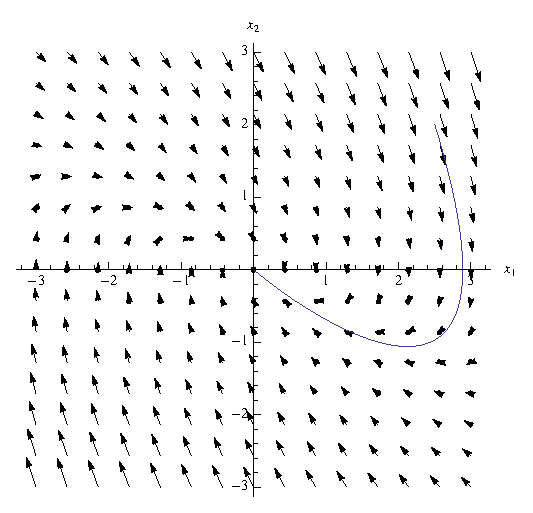
\epsfig{file=figures/phase-lyapunov.eps}
\caption{label{fig:lyapunov} A phase portrait for the system in Example~\ref{ex:lyapunov}.}
\end{figure}

\begin{example}
  The vector field for the dynamical system in
  Example~\ref{ex:lyapunov} is shown in Figure~\ref{fig:lyapunov}. The
  stability of the point $0$ is evident.\enx
\end{example}

Besides converging to a stable equilibrium, many other limiting
behaviors are possible. A system may oscillate or it may have multiple
equilibria some of which are stable and others not. 

\begin{figure}
\begin{tabular}{cc}
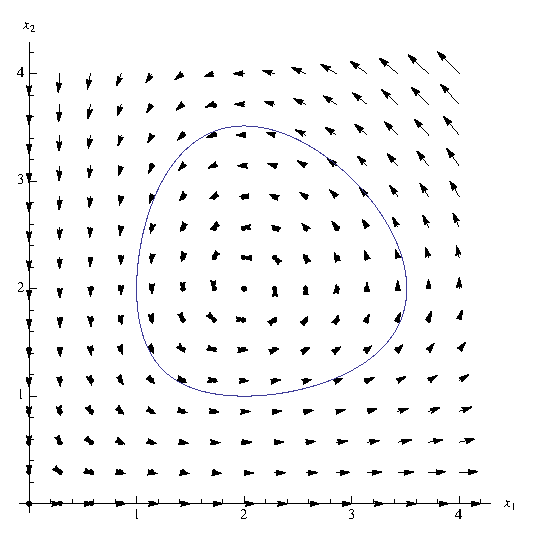
\epsfig{file=figures/osc-phase.eps, scale=0.6} & 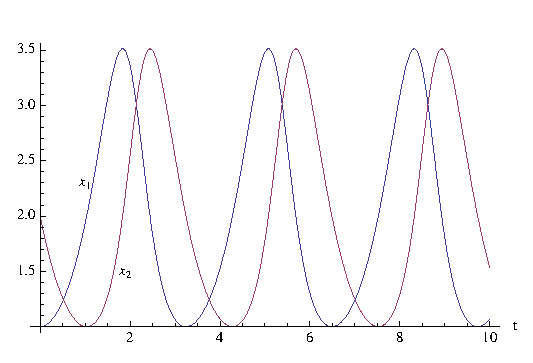
\epsfig{file=figures/osc-time.eps, scale=0.8}
\end{tabular}
\caption{\label{fig:osc} (a) Phase portrait for the system in
  Example~\ref{ex:osc}. (b) The states versus time for the same system.}
\end{figure}

\begin{example} \label{ex:osc}
A phase portrait for the system
%
\begin{eqnarray*}
\dot x_1 & = & 2 x_1 - x_1 x_2 \\
\dot x_2 & = & x_1 x_2 - 2 x_2 
\end{eqnarray*}
is shown in Figure~\ref{fig:osc}. In this system, every solution in
the right-upper quadrant is periodic.
%
\end{example}

We return to the analysis of oscillations later in the book. 

\section{Linearization and Local Stability}

A powerful tool in analyzing a dynamical system is to {\em linearize}
the system around an equilibrium. Using the Taylor series, we see that
near an equilibrium $x^*$, the system
%
\begin{equation} \label{eqn:ode-not}
\dot x = f(x) 
\end{equation}
%
becomes
%
$$
\dot x = f(x) = f(x^*) + \left . \pd f x \right |_{x=x^*} (x - x^*)
       + \mathrm{higher\ order \ terms}. 
$$
The first term in the series is zero, since $x^*$ is an
equilibrium. The higher order terms are all quadratic or higher in
$x$. The second term is the linear part of $f$ near $x^*$, called the
{\em Jacobian}, and is defined by the matrix
%
\begin{equation}\label{eqn:jac}
A = \left . \pd f x \right |_{x=x^*} = \left (
\begin{array}{ccc}
\pd{f_1}{x_1}  & \dots & \pd{f_1}{x_n} \\
\vdots & & \vdots \\
\pd{f_n}{x_1} & \dots & \pd{f_n}{x_n} 
\end{array}
\right ) .
\end{equation}
%
Thus, the dynamical system $\dot x = f(x,t)$ can be approximated, near $x^*$ by
%
\begin{equation}\label{eqn:linear}
\dot x \approx A ( x - x^* ) .
\end{equation}
%
This is of great use in understanding local stability, due to the following two results. 

\begin{theorem} \label{thm:linear-to-nonlinear} If $x^*$ is an
  asymptotically stable equilibrium of \eref{eqn:linear} then it is a
  locally asymptotically stable equilibrium of \eref{eqn:ode-not}.
\end{theorem}

\begin{theorem} [Lyapunov's Indirect
  Method] \label{thm:linear-to-nonlinear} If the real parts of the
  eigenvalues of $A$ in \eref{eqn:linear} are strictly negative, then
  the point $x^*$ a stable equilibrium of \eref{eqn:linear} and a
  locally stable equilibrium of \eref{eqn:ode-not}. 
\end{theorem}

Also, if the eigenvalues of $A$ have positive real parts, you can
conclude that the equilibrium is {\em not} stable. However, if any of
the eigenvalues have zero real parts, then the method is
inconclusive. See Exercise~\ref{exer:inconclusive}. 

\begin{example}
Consider the system 
%
\begin{eqnarray*}
\dot x_1 & = & -x_1 - x_2 + x_1 x_2 \\
\dot x_2 & = & -x_2 - x_1 x_2
\end{eqnarray*}
%
This system has two equilibra, one at $0$ and the other at
$(-1,\frac{1}{2})$. The Jacobian is
%
$$
A = \left . \left ( \begin{array}{cc}
-1 + x_2 & -1 + x_1 \\
-x_2 & -1 -x_1
\end{array}
\right ) \right |_{x=x^*}
$$
%
Evaluated at the first equilibrium, $A$ is
%
$$
A_{(0,0)} = \left ( \begin{array}{cc}
-1 & -1 \\
0 & -1
\end{array} \right )
$$
%
which has eigenvalues $-1$ and $-1$. Thus, we conclude that the point
$0$ is locally asymptotically stable. Evaluated at the second point, we get
$$
A_{(-1,\frac{1}{2})} = \left ( \begin{array}{cc}
-\frac{1}{2} & -2 \\
-\frac{1}{2} & 0
\end{array} \right )
$$
which has eigenvalues $(-1 \pm \sqrt{17})/2$: one negative and the
other positive. Thus, the second equilibrium is not stable. \enx
\end{example}

\begin{example} \label{ex:chemostat} A system that is related to the
  bacterial growth system is the {\em chemostat} in which nutrients
  are pumped into the chemostat and some bacteria and depleted
  nutrients are drained out. The new nutrient mixture effectively
  dilutes the bacteria. If we call the rate of dilution $u$ (in liters
  per minute), then the equations are
%
\begin{eqnarray}
\dot x_1 & = & \frac{v x_1 x_2}{k+x_2} - u x_1\nonumber  \\
\dot x_2 & = & - \gamma \frac{v x_1 x_2}{k+x_2} + u (n_0 - x_2 ) \label{eqn:chemostat}
\end{eqnarray}
%
where $n_0$ is the number of grams of nutrient in a liter of the input
fluid. Solving for the steady state gives two equilibria. One of these
equilibria where $x_1^(=0$, meaning that the bacteria have all been
diluted away and $x_2^*$ is simply $n_0$. To examine the conditions
under which this point is a stable equilibrium, we consider the
Jacobian at this point:
%
$$
A = \left (
\begin{array}{cc}
\frac{v }n{k+n_0}-u & 0 \\
\frac{v \gamma n_0}{k+n_0} & - u
\end{array}
\right )
$$
which has eigenvalues
$$
\lambda_1 = -u \;\; \mathrm{and} \;\; \lambda_2 = \frac{v n_0}{k+n_0} - u .
$$
%
Since $u>0$, the first of these has a negative real part. For the
second to have a negative real part, we require that
%
$$
u < \frac{v n_0}{k+n_0} \defeq u_\mathrm{max}.
$$
Thus, as long as the dilution rate is less than $u_\mathrm{max}$, the
bacteria will not get simply flushed away. \enx
%
\end{example}

% Analysis of linear systems
DISCUSSION OF 2D LINEAR SYSTEMS AND EIGENVALUES GOES HERE

\section{Non-Dimensionalization}

\section{Problems}

\setcounter{exercount}{0}

\begin{exercise}
  Show that \eref{eqn:gene-exp-sol} is the solution to
  \eref{eqn:gene-exp}.
\end{exercise}

\begin{exercise} Write the equations for protein expression with RNA
  included in the model. That is suppose that some species $R$ of RNA
  is generated by a constitutively expressed gene and that $R$ is
  translated into protein $X$. Remember that both the RNA and the
  protein will degrade. Simulate your equations and compare to the
  similar model that only includes protein. 
\end{exercise}

\begin{exercise}
Find the equilibrium points of the system
%
\begin{eqnarray*}
\dot x_1 & = & \sin x_2 \\
\dot x_2 & = & \cos x_1 .
\end{eqnarray*}
%
If you understand the idea, determine the local (asymptotic) stability
of each by linearizing around each point and finding the eigenvalues.
\end{exercise}

\begin{exercise}
  (a) Show that there are an infinite number of equilibrium points of
  the bacterial growth equations in Example~\ref{ex:growth}? (a) Which
  of the equilibria are locally stable? (c) For a given initial
  condition with $x_1(0)_0$ and $x_2(0)>0$, which particular
  equilibrium point will the system go to?
\end{exercise}

\begin{exercise}
Consider the system
%
\begin{eqnarray*}
\vvec{\dot x_1}{\dot x_2} & = & \vvec{x_2(x_1+a)}{u+\sin x_1 - a x_2} \\
\end{eqnarray*}
%
Find the equilibrium points. For each equilibrium, determin conditions
on the parameter $a$ that result in stability.
\end{exercise}

\begin{exercise}
  Linearize the following system around the point $0$ to obtain a
  linear approximation and determine the local stability of the point
  $0$.
%
\begin{eqnarray*}
\dot x_1 & = & \cos ( x_2 ) - x_1 \\
\dot x_2 & = & 2 \sin ( x_1 + x_2 ) + 3 x_1 \\
\end{eqnarray*}
\end{exercise}

\begin{exercise}
  Determine the stability of the other equilibrium point in chemostat
  system of Example~\ref{ex:chemostat} when $u > u_\mathrm{max}$. 
\end{exercise}

\begin{exercise}
  Consider the system
%
\begin{eqnarray*}
\dot x_1 & = & x_2 - x_1 ( x_1^2 + x_2^2 ) \\
\dot x_2 & = & -x_1 - x_2 ( x_1^2 + x_2^2 ) .
\end{eqnarray*}
%
(a) Show that $V = x_1^2 + x_2^2$ is a Lyapunov function showing that
$0$ is globally asymtotically stable. (b) Show that Lyapunovs indirect
method is inconclusive in this case. 
%
\end{exercise}

\begin{exercise}
Simulate the system
%
\begin{eqnarray*}
\dot x & = & - y - z \\
\dot y & = & x + 0.2 y \\
\dot z & = & 0.2 + z ( x - 5.7 )
\end{eqnarray*}
from a variety of initial conditions. Show the numerical solution
curves you obtain in 3D, all in the same plot.
%
\end{exercise}

\begin{exercise}
%
Consider the function $U(x) = cos(x)$. Find the equilibria of the system
\begin{eqnarray*}
\dot x & = & -\nabla U
\end{eqnarray*}
Determine the stability of each equilibrium. Sketch the vector field and mark the basin of attraction of each equilibrium point. 
%
\end{exercise}

\begin{exercise}
%
Repeat the previous exercise, but with
\begin{eqnarray*}
\dot x & = & v \\
\dot v & = & -\nabla U - k v
\end{eqnarray*}
For what values of $k$ does this system behave like the system in the
previous exercise?
%
\end{exercise}

\begin{exercise}
%
Consider the equations
\begin{eqnarray*}
\dot x & = & \sigma(y-x) \\
\dot y & = & x(\rho-z)-y \\
\dot z & = & x y - \beta z
\end{eqnarray*}
where $\sigma = 10$, $\rho = 28$, and $\beta = \frac{8}{3}$. Use the
software of your choice to draw the flow field of this system. Since
it is three dimensional, you can either use your software to plot it
in 3D, or project the vectors into a 2D plane (such as the $x-y$)
plane. 

Next, plot two trajectories of the system, starting at very nearby
initial conditions. What happens?
%
\end{exercise}

\begin{exercise}
%
Find chemical reactions whose dynamics match the equations in the
previous exercise.
%
\end{exercise}